\chapter{Zhodnocení a budoucí kroky}\label{zhodnocení}
V~této kapitole bude zhodnocena použitelnost aplikace v~době jejího odevzdání a navrženy vhodné budoucí kroky pro pokračování vývoje.
\section{Zhodnocení výsledné aplikace}
    Tato sekce je věnována zhodnocení použitelnosti výsledného návrhu a implementace aplikace. 
    \subsection{Implementace}
        Výsledná implementace aplikace obsahuje všechny potřebné funkce pro správné fungování, a také byly splněny všechny požadavky frontendového týmu ohledně úprav návrhu (viz kapitolu \ref{chapter:analyza}). Byla též přidána podpora dodatečných požadavků pro následné propojení Android aplikace a serverového backendu (viz kapitolu \ref{chapter:navrh}). Výsledný stav API byl kontrolován autorem frontendové části aplikace Martinem Beranem.
        Provedená implementace v~rámci této bakalářské práce je prodloužením již existující implementace. Proto pro provedené implementace s~již existující implementací byla provedena analýza na základě počtu řádků kódu aplikace. Na obrázku \ref{image:code-count-main} jsou zobrazeny výsledky analýzy.
        Pro analýzu byla uvažována jenom složka \enquote{be-springboot/src/main}. Stejná analýza byla provedena před začátkem práce pro již existující implementaci, která byla popsána v~sekci \ref{analyza:soucasnaImplementace}.
        \begin{figure}\centering
        	   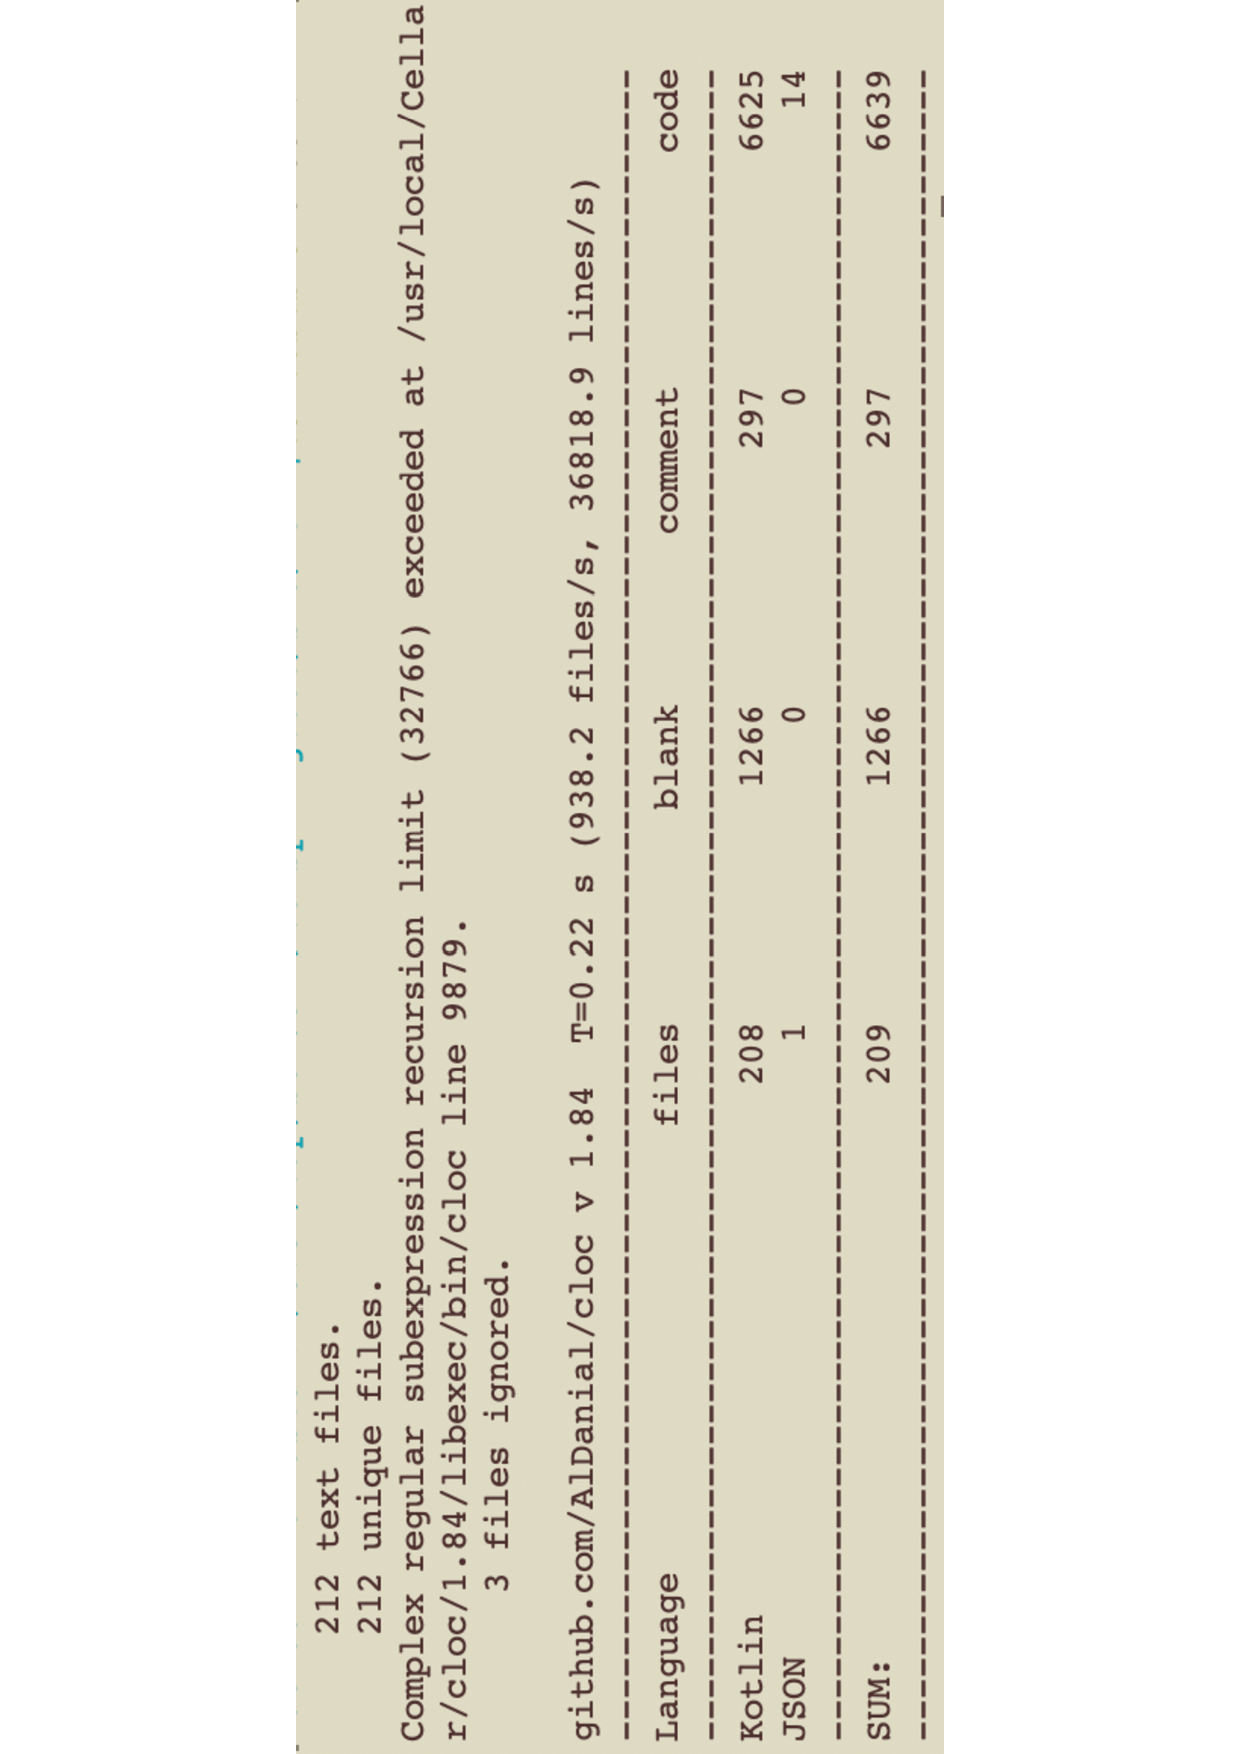
\includegraphics[angle=-90, width=0.8\textwidth]{pdfs/CodeAmountImpl2}
        	   \caption[Analýza kódu implementace]{Analýza rozsahu provedené práce za účelem implementace programu}\label{image:code-count-main}
        \end{figure}
        
        Současná implementace aplikace je funkční a je aktuálně dostupná na adrese \enquote{https://37.46.80.230/8778}. Proces nasazování aplikace byl podrobně popsán v~sekci \ref{analyza:ci}. Dokumentace API aplikace je dostupná online na adrese \enquote{https://37.46.80.230/8778/swagger-ui.html}. Výsledná verze aplikace je uložena do větve \verb|dev| v~rámci GitLab.
        Verze aplikace uložena do větve \verb|master| není aktuální, protože současná aplikace ještě není kompletně připravená pro fungování v~produkci.
        
        Pro spuštění aplikace pomocí příkazového řádku je nutné zadat příkaz \enquote{./gradlew bootRun} v~kořenové složce. Další informace o~podporovaných příkazech jsou uvedeny v~souboru \enquote{README.md}, který se také nachází v~kořenové složce. 
        
    \subsection{Testování}
        \begin{figure}\centering
    	   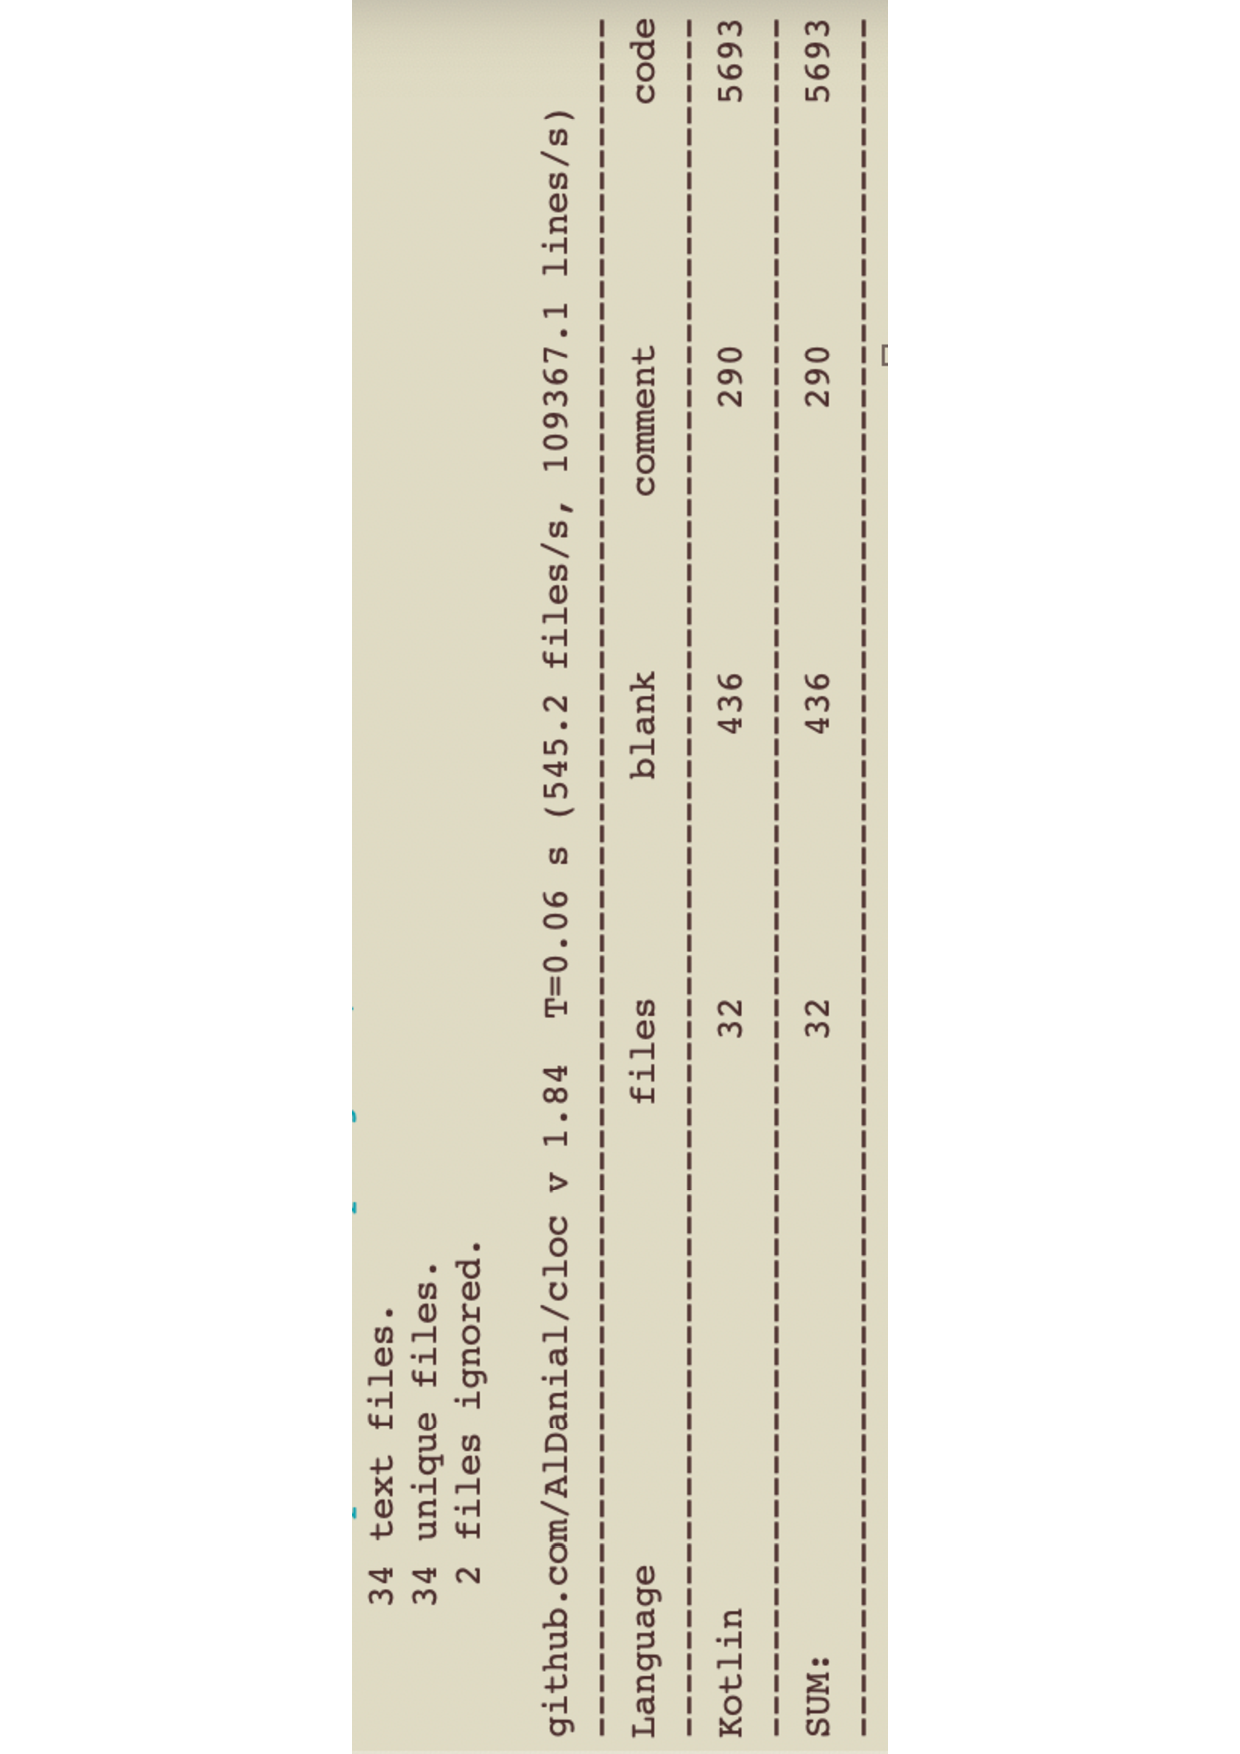
\includegraphics[angle=-90, width=0.8\textwidth]{pdfs/CodeAmountTests2}
    	   \caption[Analýza kódu testů]{Analýza rozsahu provedené práce za účelem testování programu}\label{image:code-count-test}
        \end{figure}
        Aplikace byla vhodně protestována pomocí unit testů a integračních testů (viz kapitolu \ref{chapter:testovani}). Analýza řádků kódů testování je zobrazena na obrázku \ref{image:code-count-test}. Pro spuštění testů pomocí příkazového řádku je potřeba zadat příkaz \enquote{./gradlew test} v~kořenové složce aplikace. Proces běhu testů vyžaduje specificky nastavenou databázi PostgreSQL.
        Podrobný popis požadované konfigurace bude uveden v~souboru \enquote{README.md}, který se také nachází v~kořenové složce.
    \subsection{Bezpečnost}
        Předchozí verze aplikace obsahovala jenom návrh bezpečnosti pomocí přisvojení určitých rolí každému uživateli v~rámci rodin. Tento návrh byl následně implementován a rozšířen. Proces zjištění rolí uživatele vyžadoval implementaci procesu autorizace, proto byl požít protokol OAuth 2.0. Pro zaručení bezpečné komunikace mezi klientem a serverem byl také nahrazen protokol HTTP protokolem HTTPS.
        
        V~současné implementaci je autorizační server součástí serverového backendu a odpovídá jak za registraci uživatele, tak i za přihlášení. Pro registraci má uživatel poslat DTO se svými údaje na příslušný řadič\footnote{Řadič je namapován na cestu \enquote{/api/v1/aut}.}. Pro přístup do zmíněného řadiče se používá typ přístupu \textit{user credentials}. Uživatel potřebuje uvést adresu pro obdržení \textit{tokenu}\footnote{Alfanumerické heslo.}, identifikátor uživatele a \textit{secret}. Potom uživatel obdrží \textit{tokeny} umožňující provést registraci.
        Pro přihlašování uživatele se používá typ obdržení průkazů \textit{resource owner password credetials}, kde uživatel potřebuje, navíc od předchozího typu, poslat svoje uživatelské jméno a heslo. Potom uživatel obdrží \textit{access token}\footnote{Tento \textit{token} klient používá pro komunikaci se serverem.} a \textit{refresh token}\footnote{Tento \textit{token} klient používá pro obnovení \textit{access tokenu} po vypršení jeho platnosti.} jako návratové hodnoty. Platnost \textit{tokenu} pro komunikaci je omezen jednou hodinou. Platnost \textit{tokenu} pro obnovení \textit{access tokenu} pro komunikaci je omezen jedním týdnem.
        
    \section{Požadavky na změny}
        Pro zaručení správného návrhu API je potřeba propojit výsledný návrh serverového backendu a Android aplikace, která se řeší v~rámci souběžné bakalářské práce. Proto je potřeba v~rámci této  práce připravit API, které by bylo použitelné. Současný návrh Android aplikace nepodporuje požadavky. Za účelem vyvarování kolizí výsledná implementace API serveru také nepodporuje požadavky na změny.

\section{Návrh budoucích kroků}
    Tato sekce je věnovaná návrhu vhodných budoucích kroků pro pokračování vývoje aplikace.
    
    \subsection{Testování}
        Výsledný stav backendové části aplikace je připraven k~použití současným stavem fronendové části aplikace. API serveru bylo kontrolováno autorem souběžně vyvíjenou frontedovou částí aplikace. Pro následující proces vývoje nastavení Android aplikace mají být upraveny pro použití externího serveru. Po provedených úpravách má být provedeno podrobné testování, jestli jsou všechny funkce implementovány správně a případně opraveny.
    
    \subsection{Implementace}
        Po úspěšném propojení serverového backendu a souběžně vyvíjené Android aplikace má být dokončen implementace chybějících funkcí. Do takových funkcí patří požadavky na změny v~rámci rodiny. 
        
    \subsection{Bezpečnost}
        V~současné implementaci aplikace je autorizační server součástí serverového backendu. Proto, pro zvýšení bezpečnosti aplikace, je nutné přidat možnost přihlašování pomocí externího autorizačního serveru. Proces přihlašování se potom změní následujícím způsobem: klient se přihlásí do autorizačního serveru a obdrží \textit{access token} a \textit{refresh token}. 
        Tyto \textit{tokeny} klient potom může použít pro komunikaci se serverem. Server bude ověřovat platnost \textit{tokenů} dotazováním na externí autorizační server.
